\chapter{Il nucleo di un sistema multiprogrammato (modello a memoria comune)}

\subsection{Nucleo di un sistema a processi}
In un sistema multiprogrammato, vengono offerte tante unità di elaborazione astratte quanti sono i processi. Ogni macchina possiede tutte le istruzioni elementari dell'unità centrale, più alcune irate alla gestione dei processi, alla comunicazione e sincronizzazione.

Questo modello mette in evidenza le proprietà logiche di comunicazione e sincronizzazione senza pensare agli aspetti implementativi.

\begin{mdframed}[topline=false,bottomline=false,rightline=false]
Si chiama \textbf{kernel} (nucleo) il modulo realizzato in software o firmware che supporta il concetto di processo e realizza gli strumenti necessari per la gestione di questi ultimi.
\end{mdframed}

Il nucleo è l'unico componente del sistema che è "conscio" dell'esistenza delle \textbf{interruzioni}:
ogni processo che richiede l'esecuzione di una operazione a un dispositivo effettua una chiamata primitiva al nucleo che lo \textit{sospende}, quest ultimo riceve un \textit{segnale di interruzione} dal dispositivo e risveglia il processo sospeso.

La gestione delle interruzioni è invisibile ai processi.

\subsection{Stati di un processo}

\begin{multicols}{2}
\begin{multicolfigure}
    \centering
    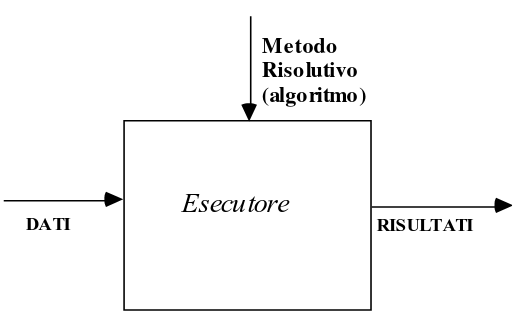
\includegraphics[width=\textwidth]{/home/riccardoob/appunti/sistemi_operativi/images/26.png}
\end{multicolfigure}
\columnbreak
\begin{multicolfigure}
    \centering
    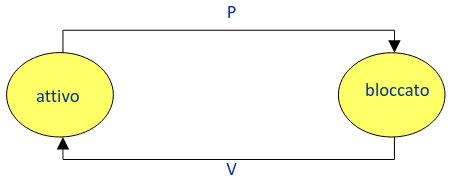
\includegraphics[width=\textwidth]{/home/riccardoob/appunti/sistemi_operativi/images/27.png}
\end{multicolfigure}    
\end{multicols}

\begin{mdframed}[topline=false,bottomline=false,rightline=false]
\textbf{Contesto di un processo}\\
Insieme delle informazioni contenute nei registri del processore, quando esso opera sotto il controllo del processo.
\end{mdframed}

\begin{mdframed}[topline=false,bottomline=false,rightline=false]
\textbf{Salvataggio di contesto}\\
Quando un processo perde il controllo del processore, il contenuto dei registri del processore (contesto) viene salvato in una struttura dati associata al processo, chiamata \textbf{descrittore}.
\end{mdframed}

\begin{mdframed}[topline=false,bottomline=false,rightline=false]
\textbf{Ripristino del contesto}\\
Quando un processo viene schedulato, i valori salvati nel suo descrittore vengono caricati nei registri del processore.
\end{mdframed}

\subsection{Funzioni del nucleo}
Il compito fondamentale del nucleo è quello di \textbf{gestire le transizione di stato} dei processi, in particolare:
\begin{itemize}
    \item gestione del \textbf{salvataggio} e \textbf{ripristino} dei \textit{contesti} dei processi
    \item scelta, tra i processi pronti, del processo al quale assegnare l'unità di elaborazione (\textbf{scheduling}, secondo una particolare poitica (FIFO, SJF, Priorità etc.)
    \item gestione delle interruzioni dei dispositivi esterni
    \item realizzazione dei meccanismi di sincronizzazione dei processi
\end{itemize}

\subsection{Caratteristiche del nucleo}
\begin{mdframed}[topline=false,bottomline=false,rightline=false]
\textbf{Efficienza}\\
Dato che condiziona l'intera struttura a processi, in certi sistemi alcune funzionalità sono realizzate in hardware o microprogrammi.
\end{mdframed}

\begin{mdframed}[topline=false,bottomline=false,rightline=false]
\textbf{Dimensioni}\\
Necessità di avere un nucleo semplice e di dimensione limitata.
\end{mdframed}

\begin{mdframed}[topline=false,bottomline=false,rightline=false]
\textbf{Separazione meccanismi e politiche}\\
Il nucleo deve contenere, possibilmente, soltanto meccanismi, consentendo così a livello di processo di utilizzare tali meccanismi ad hoc.
\end{mdframed}

\section{Realizzazione del nucleo (monoprocessore)}

\subsection{Strutture dati del nucleo}

\subsubsection{Descrittore del processo}

Contiene le seguenti informazioni
\begin{itemize}
    \item \textbf{identificatore} del processo, univoco
    \item \textbf{stato} del processo: pronto, esecuzione, bloccato etc.
    \item modalità di \textbf{servizio} dei processi: parametri di scheduling, ad esempio
    \begin{itemize}
        \item FIFO
        \item Priorità
        \item Deadline (completamento richiesta processo)
        \item quanto di tempo
    \end{itemize}
    \item \textbf{contesto} del processo: \textit{contatore} di programma, \textit{registro di stato}, registri generali, indirizzo memoria privata del processo
    \item riferimenti a \textbf{code}: riferimento elemento successivo nella coda (di processi bloccati, di processi pronti...)
\end{itemize}

\begin{minted}[bgcolor=lightgray,framesep=2mm,baselinestretch=1.2,fontsize=\footnotesize]{c}
typedef struct {
    int indice_priorità;
    int delta_t;
} modalita_di_servizio;

typedef struct {
    int nome;
    ...
    modalita_di_servizio servizio;
    tipo_contesto contesto;
    tipo_stato stato;
    int successivo;
} descrittore_processo;
\end{minted}

\subsubsection{Coda dei processi pronti}
Esistono diverse code di \textit{processi pronti}, quando un processo è riattivato da un V, viene inserito in fondo alla coda corrispondente alla sua priorità.

Non sempre è presente un processo pronto, però esiste un \textbf{dummy processo} che va in esecuzione quanto tutte le altre code sono vuote, rimanendoci fino a un altro processo diventa pronto, ha la priorità più bassa ed è sempre in stato pronto.

\begin{minted}[bgcolor=lightgray,framesep=2mm,baselinestretch=1.2,fontsize=\footnotesize]{c}
typedef struct {
    int primo, ultimo;
} descrittore_coda;

typedef descrittore_coda coda_a_livelli[Npriorità];
\end{minted}

\begin{multicols}{2}
\begin{multicolfigure}
    \centering
    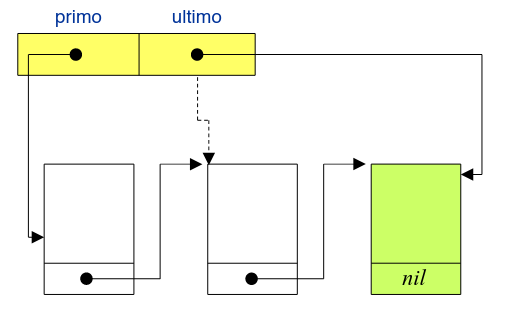
\includegraphics[width=\textwidth]{/home/riccardoob/appunti/sistemi_operativi/images/28.png}
\end{multicolfigure}
\columnbreak
\begin{minted}[bgcolor=lightgray,framesep=2mm,baselinestretch=1.2,fontsize=\footnotesize]{c}
void Inserimento(int P,
                 descrittore_coda C) {
    //inserimento processo di indice P
    //nella coda C
}
\end{minted}
    
\end{multicols}
\begin{multicols}{2}
\begin{multicolfigure}
    \centering
    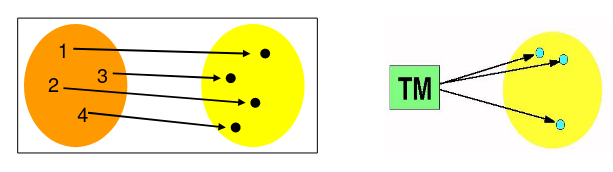
\includegraphics[width=\textwidth]{/home/riccardoob/appunti/sistemi_operativi/images/29.png}
\end{multicolfigure}
\columnbreak
\begin{minted}[bgcolor=lightgray,framesep=2mm,baselinestretch=1.2,fontsize=\footnotesize]{c}
int Prelievo(descrittore_coda C) {
    //estrae il primo processo da coda
    //C e restituisce l'indice
}
\end{minted} 
\end{multicols}

\subsubsection{Coda dei descrittori liberi}
In questa coda sono contenuti i descrittori \textit{disponibili} per la creazione di nuovi processi, vengono reinseriti i descrittori dei processi terminati.

\begin{minted}[bgcolor=lightgray,framesep=2mm,baselinestretch=1.2,fontsize=\footnotesize]{c}
descrittore_coda descrittori_liberi;
\end{minted}

\subsubsection{Processo in esecuzione}
Il nucleo necessita di tenere traccia di quale processo è in esecuzione, informazione rappresentata dall'indice del descrittore del processo, viene salvato in una variabile del nucleo (spesso un registro del processore)
\begin{minted}[bgcolor=lightgray,framesep=2mm,baselinestretch=1.2,fontsize=\footnotesize]{c}
int processo_in_esecuzione;
\end{minted}

\subsection{Funzioni del nucleo}
Le funzioni del nucleo implementano le operazioni di \textbf{transizione di stato} per i singoli processi, ogni transizione prevede il \textit{prelievo} da una coda e l'\textit{inserimento} in un'altra.

Se la coda è vuota, essa contiene soltanto il valore -1 (NIL), valore inserito anche in code non vuote come ultimo elemento.

\subsubsection{Struttura del nucleo}
La struttura del nucleo si articola in due livelli:
\begin{itemize}
    \item \textbf{livello superiore}: contiene tutte le funzioni direttamente \textbf{utilizzate dai processi}, sia interni che esterni; in particolare le primitive per la creazione, eliminazione e sincronizzazione dei processi e le funzioni di risposta ai segnali di interruzione
    \item \textbf{livello inferiore}: realizza le funzionalità di \textbf{cambio di contesto}: salvataggio del contesto del processo deschedulato, scelta di un nuovo processo da mettere in esecuzione tra quelli pronti e ripristino del suo contesto
\end{itemize}

\subsubsection{Esecuzione del kernel}
Le funzioni del nucleo, per motivi di protezione, sono le sole che possono operare su strutture dati dello stato del sistema e utilizzare istruzioni privilegate.

Grazie al meccanismo dei \textbf{ring}, nucleo e processi eseguono in due \textbf{ambienti separati}:
\begin{itemize}
    \item \textit{nucleo}, massimo privilegio: \textbf{modo kernel} o ring 0
    \item \textit{processi}, minore privilegio: \textbf{modo user} o ring > 0
\end{itemize}

Il passaggio da un "modo" all'altro è basato sul \textit{meccanismo delle interuzioni}:
\begin{itemize}
    \item funzioni da processi \textbf{esterni}: passaggio ad ambiente nucleo tramite risposta al segnale di \textbf{interruzione}
    \item funzioni da processi \textbf{interni}: passaggio ad ambiente nucleo tramite \textbf{system calls} (SVC, interruzioni interne)
\end{itemize}

In entrambi i casi al completamento della funzione, il trasferimento avviene tramite il meccanismo di \textbf{ritorno da interruzione} (RTI).

\subsubsection{Funzioni del livello inferiore}
Le funzioni principali di \textbf{cambio di contesto} sono
\begin{itemize}
    \item \texttt{salvataggio\_stato}: salvataggio del contesto del processo in esecuzione e inserimento del descrittore nella coda dei processi bloccati o pronti
    \item \texttt{assegnazione\_cpu}: rimozione del processo a maggior priorità dalla coda e caricamento dell'identificatore nel registro del processo in esecuzione
    \item \texttt{ripristino\_stato}: caricamento del contesto del nuovo processo nei registri di macchina
\end{itemize}

\begin{minted}[bgcolor=lightgray,framesep=2mm,baselinestretch=1.2,fontsize=\footnotesize]{c}
void salvataggio_stato() {
    int j;
    j = process_in_esecuzione;
    descrittori[j].contesto = <valori dei registri CPU>;
}

void ripristino_stato() {
    int j;
    j = processo_in_esecuzione;
    <registro-temp> = descrittori[j].servizio.delta_t;
    <registri-CPU> = descrittori[j].contesto;
}

void assegnazione_CPU() { //scheduling: hp algoritmo con priorità
    int k = 0, j;
    while ((coda_processi_pronti[k].primo) == -1) {
        k++;
    }
    j = prelievo(coda_processi_pronti[k]);
    processo_in_esecuzione = j;
}
\end{minted}

\subsubsection{Gestione del temporizzatore}
Per consentire la modalità di servizio a divisione del tempo è necessario che il nucleo gestisca un \textbf{dispositivo temporizzatore} tramite una apposita procedura che ad intervalli di tempo fissati, provveda a sospendere il processo in esecuzione ed assegnare l'unità di elaborazione ad un altro processo.

\begin{minted}[bgcolor=lightgray,framesep=2mm,baselinestretch=1.2,fontsize=\footnotesize,escapeinside=||,mathescape=true]{c}
void cambio_contesto() {
    int j, k;
    salvataggio_stato();
    j = processo_in_esecuzione;
    k = descrittori[j].servizio.priorità;
    inserimento(j, coda_processi_pronti[k]);
    assegnazione_CPU();
    ripristino_stato();
}
\end{minted}

\section{Realizzazione del semaforo (monoprocessore)}

\subsection{Semafori}

Nel nucleo di un sistema monoprocessore il semaforo può essere implementato tramite:
\begin{itemize}
    \item una \textit{variabile intera} che rappresenta il suo valore (\texttt{>= 0})
    \item una \textit{coda di decrittori} dei processi in attesa sul semaforo
\end{itemize}

Se non ci sono processi in coda, il puntatore contiene costante \texttt{NIIL}.

La coda viene gestita con politica FIFO, un descrittore viene inserito nella coda come risultato dei una \texttt{P} bloccante e viene prelevato per effetto di una \texttt{V}.

\begin{minted}[bgcolor=lightgray,framesep=2mm,baselinestretch=1.2,fontsize=\footnotesize,escapeinside=||,mathescape=true]{c}
typedef struct {
    int contatore;
    descrittore_coda coda;
} descr_semaforo;
\end{minted}

\subsubsection{Operazione P}
\begin{figure}[H]
    \centering
    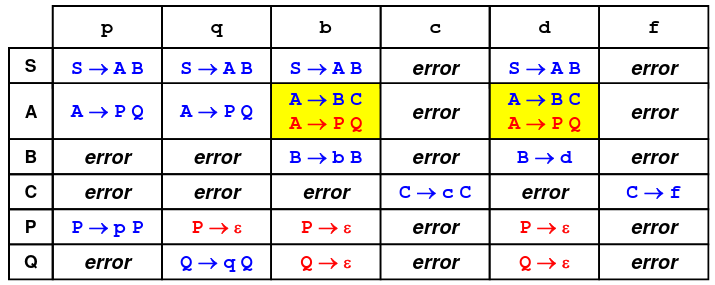
\includegraphics[width=0.7\textwidth]{/home/riccardoob/appunti/sistemi_operativi/images/31.png}
\end{figure}

\begin{minted}[bgcolor=lightgray,framesep=2mm,baselinestretch=1.2,fontsize=\footnotesize,escapeinside=||,mathescape=true]{c}
// insieme di tutti i semafori
descr_semaforo semafori[num_max_sem];
// ogni semaforo è rappresentato dall'indice che lo individua nel vettore

typedef int semaforo;

void P(semaforo s) {
    int j, k;
    if (semafori[s].contatore == 0) {
        salvataggio_stato();
        j = processo_in_esecuzione;
        inserimento(j, semafori[s].coda);
        assegnazione_CPU(); // scheduling
        ripristino_stato();
    }
    else 
        contatore--;
}
\end{minted}

\subsubsection{Operazione V}
\begin{figure}[H]
    \centering
    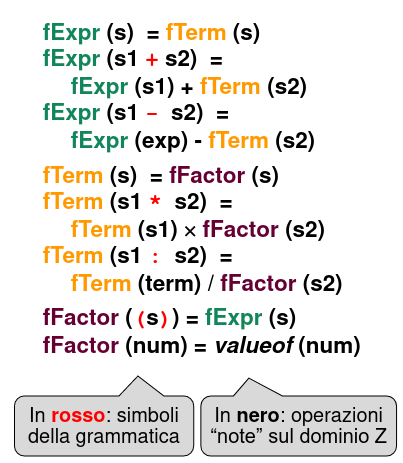
\includegraphics[width=0.7\textwidth]{/home/riccardoob/appunti/sistemi_operativi/images/32.png}
\end{figure}

\begin{minted}[bgcolor=lightgray,framesep=2mm,baselinestretch=1.2,fontsize=\footnotesize,escapeinside=||,mathescape=true]{c}
void V(semaforo s) {
    // j, k processi -- p, q indici priorità
    int j, k, p, q;
    
    if (semafori[s].coda.primo != -1) { // la coda non è vuota
        k = prelievo(semafori[s].coda);
        j = processo_in_esecuzione;
        p = descrittori[j].servizio.priorità; // priorità proc running
        q = descrittori[k].servizio.priorità; // priorità proc risvegliato

        if (p > q) // processo running ha priorità
            inserimento(k, coda_processi_pronti[q]);
        else {
            salvataggio_stato();
            inserimento(j, coda_processi_pronti[p]);
            processo_in_esecuzione = k;
            ripristino_stato();
        }
    }
    else
        semafori[s].contatore++; // se non ci sono processi in coda
}           
\end{minted}

\section{Realizzazione del nucleo (multiprocessore)}

\subsubsection{Architettura}
\begin{figure}[H]
    \centering
    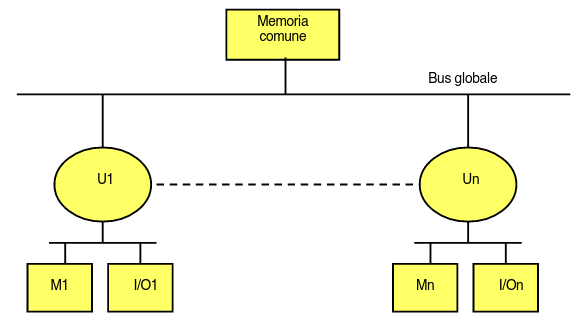
\includegraphics[width=0.7\textwidth]{/home/riccardoob/appunti/sistemi_operativi/images/33.png}
\end{figure}

\subsubsection{Modelli principali}
Un OS che esegue su una architettura multiprocessore deve gestire \textbf{molteplici CPU}, le quali possono tutte accedere a una \textbf{memoria condivisa}.

Esistono due modelli:
\begin{itemize}
    \item modello \textbf{SMP}: unica copia del nucleo, condivisa tra tutte le CPU
    \item modello \textbf{nuclei distinti}: più istanze concorrente del nucleo
\end{itemize}

\section{Modello SMP - Symmetric Multi Processing}
Nel modello SMP, esiste una \textit{unica copia del nucleo} del sistema operativo, allocata nella memoria comune e si occupa della gestione di tutte le risorse disponibili, comprese le CPU.

Caratteristiche:
\begin{itemize}
    \item ogni processo può essere allocato su \textit{una qualunque} delle CPU
    \item la system call richieste dai processi possono essere contemporanee, è necessario che gli accessi al nucleo avvengano in modo \textbf{sincronizzato}, in quanto in generale è richiesto l'accesso a strutture dati interne
\end{itemize}

\subsection{Sincronizzazione nell'accesso al nucleo}

\subsubsection{Soluzione singolo lock}
Viene associato un lock \texttt{L} al nucleo, per garantire la mutua esclusione dell'esecuzione di funzioni del nucleo: si sincronizza l'accesso alle strutture dati eseguendo \texttt{lock} e \texttt{unlock} sull'unico lock \texttt{L}.

Il problema fondamentale di questa soluzione è la vasta \textit{limitazione del grado di parallelismo}, escludendo operazioni che accedono a strutture dati distinte.

\subsubsection{Soluzione molteplici lock}
Un grado maggiore di parallelismo si può ottenere individuando \textit{classi} di sezioni critiche, ognuna associata a una struttura sufficientemente indipendente dalle altre, a ogni struttura dati viene associato un \textbf{lock distinto}.

\subsection{Scheduling dei processi}
Il modello SMP consente la schedulazione di ogni processo su uno qualunque dei processori, con la possibilità di attuare politiche \textbf{load balancing} sul carico dei diversi processori.

Esistono casi in cui conviene assegnare un processo a un \textit{determinato processore}:
\begin{itemize}
    \item schedulare il processo a un processore che contiene il codice nella sua memoria privata (accesso più veloce)
    \item sistemi NUMA accedono alla memoria più "vicina" più velocemente, quindi conviene schedulare il processo a un processore più vicino alla memoria contenente lo spazio di indirizzamento
    \item in caso di presenza di memoria cache (es. TLB memoria virtuale) può essere utile schedulare su un processore precedentemente usato per un particolare processo
\end{itemize}

\section{Modello a nuclei distinti}



















































































































